\documentclass[../general/general]{subfiles}


\begin{document}

\chapter{Лекция №4}
\noindent\textit{А.\,М.~Белемук \hfill 6 марта 2021}
\vspace{1em}



% --- SECTION: Напоминание: Статистический оператор канонического ансамбля ---
\section{Напоминание: Статистический оператор канонического ансамбля}

% --- SUBSECTION: Вид статистического оператора и статистическая сумма ---
\subsection{Вид статистического оператора и статистическая сумма}

Ну что, у нас сегодня лекция четвертая. Тему лекции я напишу чуть позже, а пока мы продолжим то, что рассматривалось на лекции номер три. Мы продолжаем изучать статистический оператор, который мы ввели для канонического распределения.

Мы с вами увидели, что статистический оператор $\hat{\rho}$, определяемый как сумма по всем квантовым состояниям от вероятности $w_k$ найти систему в $k$-том квантовом состоянии, умноженной на соответствующий проектор:
\begin{equation*}
    \hat{\rho} = \sum_k w_k |\Psi_k\rangle \langle \Psi_k|
\end{equation*}
у нас благополучно свернулся в следующий оператор:
\begin{equation}
    \hat{\rho} = \frac{1}{Z} e^{-\frac{\hat{H}}{T}}
    \label{eq:rho_canonical}
\end{equation}
Это и есть вид статистического оператора для канонического распределения. На этом мы остановились в прошлый раз, и теперь давайте сделаем небольшие дополнения.

Поскольку мы знаем, что шпур (след) матрицы плотности (или статистического оператора) равен единице:
\begin{equation*}
    \operatorname{Sp}\hat{\rho} = 1
\end{equation*}
Подставляя выражение для оператора из формулы \eqref{eq:rho_canonical}, мы можем записать:
\begin{equation*}
    \frac{1}{Z} \operatorname{Sp} \left( e^{-\frac{\hat{H}}{T}} \right) = 1
\end{equation*}
Множитель $1/Z$ — это просто число, поэтому мы имеем полное право вынести его из-под знака шпура. Следовательно, из этого условия нормировки немедленно вытекает выражение для статистической суммы $Z$ в квантовой статистике:
\begin{equation}
    Z = \operatorname{Sp} \left( e^{-\frac{\hat{H}}{T}} \right)
    \label{eq:Z_quantum}
\end{equation}

Итак, запоминаем формулу \eqref{eq:rho_canonical} для статистического оператора и формулу \eqref{eq:Z_quantum} для статистической суммы. Эти два соотношения будут очень интенсивно использоваться в нашем курсе в дальнейшем.



% --- SECTION: Флуктуации энергии в каноническом ансамбле ---
\section{Флуктуации энергии в каноническом ансамбле}

А теперь следующий пункт: мы закончили формальное введение статистического оператора, и давайте рассмотрим флуктуации энергии в каноническом ансамбле. 

% --- SUBSECTION: Распределение системы по состояниям с разной энергией ---
\subsection{Распределение системы по состояниям с разной энергией}

Смотрите, у нас есть система, которая с разными вероятностями $w_k$ находится в различных микроскопических квантовых состояниях. Каждое такое состояние $\Psi_k$ (которое является собственной функцией гамильтониана) имеет свою собственную энергию $E_k$. 

Поэтому, вообще говоря, с разной вероятностью наша система находится в состояниях с разной энергией. Следовательно, те значения энергии $E$, которые мы можем обнаружить у системы (так как она обменивается теплом с термостатом), как-то распределены. Они распределены около некоторого среднего значения, которое мы обозначаем как $\langle E \rangle$. Это среднее значение в термодинамике мы называем просто термодинамической внутренней энергией и обычно пишем просто букву $E$ без скобок усреднения.

Итак, энергия системы, обменивающейся теплом с термостатом, флуктуирует около некоторого среднего значения. Давайте посчитаем, как сильно она флуктуирует и насколько велики эти отклонения.

% --- SUBSECTION: Введение меры флуктуаций (среднеквадратичное отклонение) ---
\subsection{Введение меры флуктуаций (среднеквадратичное отклонение)}

Мерой таких отклонений, или мерой флуктуаций, обычно служит среднеквадратичное отклонение. Обозначим его как $\langle \Delta E^2 \rangle$. По определению из теории вероятностей, средний квадрат флуктуации равен разности среднего квадрата энергии и квадрата средней энергии:
\begin{equation}
    \langle \Delta E^2 \rangle = \langle E^2 \rangle - \langle E \rangle^2
    \label{eq:energy_dispersion_def}
\end{equation}
Давайте посмотрим на каждое из этих слагаемых. Очевидно, что средняя энергия $\langle E \rangle$ вычисляется как сумма по всем квантовым состояниям от энергии состояния, умноженной на вероятность этого состояния:
\begin{equation*}
    \langle E \rangle = \sum_k E_k w_k
\end{equation*}
Напомним, что вероятность $w_k$, фигурирующая в распределении Гиббса, имеет вид:
\begin{equation*}
    w_k = \frac{1}{Z} e^{-\frac{E_k}{T}}
\end{equation*}
где $Z$ — статистическая сумма.

Аналогично, среднее от квадрата энергии вычисляется по формуле:
\begin{equation*}
    \langle E^2 \rangle = \sum_k E_k^2 w_k = \sum_k E_k^2 \frac{1}{Z} e^{-\frac{E_k}{T}}
\end{equation*}

% --- SUBSECTION: Вычисление среднего квадрата энергии ---
\subsection{Вычисление среднего квадрата энергии}

Можно было бы по отдельности вычислить $\langle E^2 \rangle$ и $\langle E \rangle^2$, а затем взять их разность. Но можно немного схитрить, чтобы сразу получить искомую флуктуацию.

Мы знаем из предыдущих лекций полезную математическую операцию. Мы уже видели, что применение дифференциального оператора $T^2 \frac{\partial}{\partial T}$ к логарифму статсуммы дает нам среднюю энергию:
\begin{equation}
    T^2 \frac{\partial}{\partial T} \ln Z = \langle E \rangle
    \label{eq:mean_E_derivative}
\end{equation}

% --- SUBSECTION: Применение оператора производной по температуре ---
\subsection{Применение оператора производной по температуре}

Посмотрим, что эта операция даст, если мы применим её уже не к логарифму статсуммы, а сразу к самой средней энергии $\langle E \rangle$. Раз эта операция оказалась такой полезной, давайте применим её еще раз. Вычислим величину $T^2 \frac{\partial}{\partial T} \langle E \rangle$:
\begin{equation*}
    T^2 \frac{\partial}{\partial T} \langle E \rangle = T^2 \frac{\partial}{\partial T} \left( \sum_k E_k \frac{1}{Z} e^{-\frac{E_k}{T}} \right)
\end{equation*}
Поскольку оператор производной линейный, мы можем внести его под знак суммы, учитывая, что от температуры $T$ зависят как статсумма $Z$, так и экспоненциальный множитель. Перепишем это, вынеся функцию $1/Z$ и экспоненту как произведение:
\begin{equation*}
    T^2 \frac{\partial}{\partial T} \langle E \rangle = T^2 \frac{\partial}{\partial T} \left( \frac{1}{Z} \sum_k E_k e^{-\frac{E_k}{T}} \right)
\end{equation*}

Сначала дифференцируем первый множитель $1/Z$. Производная по $T$ даст:
\begin{equation*}
    \frac{\partial}{\partial T} \left( \frac{1}{Z} \right) = -\frac{1}{Z^2} \frac{\partial Z}{\partial T}
\end{equation*}
Домножая это на $T^2$ и на оставшуюся сумму, получаем первое слагаемое:
\begin{equation*}
    -T^2 \frac{1}{Z^2} \frac{\partial Z}{\partial T} \sum_k E_k e^{-\frac{E_k}{T}}
\end{equation*}

Затем дифференцируем по $T$ саму экспоненту, оставляя $1/Z$ в покое:
\begin{equation*}
    T^2 \frac{1}{Z} \sum_k E_k \frac{\partial}{\partial T} \left( e^{-\frac{E_k}{T}} \right) = T^2 \frac{1}{Z} \sum_k E_k e^{-\frac{E_k}{T}} \left( \frac{E_k}{T^2} \right)
\end{equation*}

Теперь упростим оба полученных слагаемых. Начнем с первого:
\begin{equation*}
    - \left( T^2 \frac{1}{Z} \frac{\partial Z}{\partial T} \right) \left( \frac{1}{Z} \sum_k E_k e^{-\frac{E_k}{T}} \right)
\end{equation*}
Заметим, что дробь $\frac{1}{Z} \frac{\partial Z}{\partial T}$ — это производная логарифма $\frac{\partial \ln Z}{\partial T}$. Таким образом, выражение в первых скобках равно $T^2 \frac{\partial \ln Z}{\partial T}$, что в точности есть средняя энергия $\langle E \rangle$. Выражение во вторых скобках — это снова определение средней энергии $\langle E \rangle$. Итого, первое слагаемое дает нам:
\begin{equation*}
    -\langle E \rangle \langle E \rangle = -\langle E \rangle^2
\end{equation*}

Перейдем ко второму слагаемому:
\begin{equation*}
    T^2 \frac{1}{Z} \sum_k E_k \left( \frac{E_k}{T^2} \right) e^{-\frac{E_k}{T}}
\end{equation*}
Температура $T^2$ в числителе и знаменателе благополучно сокращается. Остается:
\begin{equation*}
    \frac{1}{Z} \sum_k E_k^2 e^{-\frac{E_k}{T}}
\end{equation*}
А это, по определению, есть среднее от квадрата энергии $\langle E^2 \rangle$.

Собирая результаты вместе, мы приходим к замечательному соотношению:
\begin{equation}
    T^2 \frac{\partial \langle E \rangle}{\partial T} = \langle E^2 \rangle - \langle E \rangle^2 = \langle \Delta E^2 \rangle
\end{equation}
Вся эта операция очень полезна, так как она сразу выдала нам среднеквадратичную флуктуацию энергии.

% --- SUBSECTION: Связь дисперсии энергии с макроскопической теплоемкостью ---
\subsection{Связь дисперсии энергии с макроскопической теплоемкостью}

Давайте теперь посмотрим, как связана полученная производная с макроскопическими термодинамическими величинами. Нам нужно вычислить $\frac{\partial \langle E \rangle}{\partial T}$. 

Примем во внимание, какими переменными характеризуется наш канонический ансамбль. Канонический ансамбль описывается фиксированными объемом $V$, числом частиц $N$ и температурой $T$, задаваемой термостатом. Поэтому, когда мы берем частную производную от средней энергии по температуре, мы подразумеваем, что объем и число частиц фиксированы:
\begin{equation*}
    \left( \frac{\partial \langle E \rangle}{\partial T} \right)_{V, N}
\end{equation*}
Что это за величина? Вспомним термодинамику. Теплоемкость при постоянном объеме и числе частиц по определению равна:
\begin{equation*}
    C_V = \left( \frac{\delta Q}{dT} \right)_{V, N} = T \left( \frac{\partial S}{\partial T} \right)_{V, N}
\end{equation*}
Поскольку объем постоянен, работа не совершается ($dV = 0$), и переданное тепло полностью идет на изменение внутренней энергии ($dQ = dE$). Следовательно, теплоемкость $C_V$ в точности равна производной внутренней энергии по температуре:
\begin{equation*}
    C_V = \left( \frac{\partial \langle E \rangle}{\partial T} \right)_{V, N}
\end{equation*}
Подставляя это в выражение для флуктуации, мы делаем важный вывод: средний квадрат флуктуации энергии системы, находящейся в контакте с термостатом, прямо пропорционален ее теплоемкости:
\begin{equation}
    \langle \Delta E^2 \rangle = T^2 C_V
    \label{eq:energy_fluctuation_CV}
\end{equation}
Это еще один фундаментальный результат статистической физики.

% --- SUBSECTION: Относительная флуктуация энергии в термодинамическом пределе ---
\subsection{Относительная флуктуация энергии в термодинамическом пределе}

Спрашивается, много это или мало? Допустим, мы посчитали флуктуацию и получили, например, величину порядка миллиона джоулей в квадрате. С чем нам нужно сравнивать это значение, чтобы понять физический масштаб отклонений?

Естественно, абсолютную флуктуацию необходимо сравнивать со средним значением самой величины. Давайте оценим относительную флуктуацию:
\begin{equation*}
    \text{Относительная флуктуация} = \frac{\sqrt{\langle \Delta E^2 \rangle}}{\langle E \rangle}
\end{equation*}
Вспомним свойства экстенсивности. Внутренняя энергия системы $\langle E \rangle$ пропорциональна числу частиц: $\langle E \rangle \sim N$. Теплоемкость системы $C_V$ также является экстенсивной величиной и пропорциональна числу частиц: $C_V \sim N$.

Тогда для относительной флуктуации мы получаем оценку:
\begin{equation*}
    \frac{\sqrt{\langle \Delta E^2 \rangle}}{\langle E \rangle} \sim \frac{\sqrt{N}}{N} = \frac{1}{\sqrt{N}}
\end{equation*}
При переходе к термодинамическому пределу, когда число частиц $N \to \infty$ (для макроскопических систем порядка $10^{23}$), эта величина стремится к нулю. Это означает, что для макроскопических систем относительные флуктуации энергии ничтожно малы. 

% --- SUBSECTION: Функция распределения по энергиям и эквивалентность ансамблей ---
\subsection{Функция распределения по энергиям и эквивалентность ансамблей}

Если мы рассмотрим функцию распределения $W(E)$, которая определяет вероятность найти нашу систему в заданном интервале энергий от $E$ до $E+dE$, мы получим весьма характерную картину.

%[ТАЙМКОД 17:05-18:00: График функции распределения по энергиям W(E) с узким пиком около <E>]
\begin{center}
    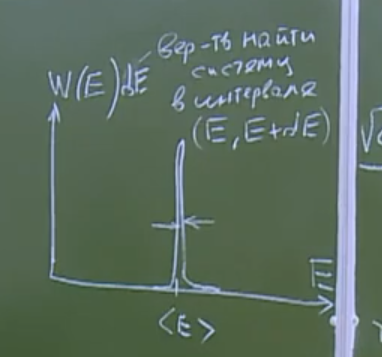
\includegraphics[width=0.4\textwidth]{images/1.png}
\end{center}

Если мы нарисуем этот график, то по оси абсцисс будет отложена энергия $E$, а по оси ординат — вероятность $W(E)$. Из-за того, что относительные флуктуации стремятся к нулю, эта вероятность будет сосредоточена в виде очень-очень узкого пика вблизи среднего значения $\langle E \rangle$. 

Подавляющая часть распределения локализована в узкой области. Если мы не находимся вблизи точки фазового перехода (где флуктуации могут аномально возрастать), мы можем пренебречь этими флуктуациями. В термодинамических расчетах мы с полным правом можем полагать, что истинная энергия системы совпадает со средней: $E \approx \langle E \rangle$. 

В этом смысле канонический ансамбль (система, обменивающаяся энергией с термостатом) полностью эквивалентен микроканоническому ансамблю (строго изолированной системе) в термодинамическом пределе. Все предсказания для термодинамических функций в обоих случаях будут идентичны. Сам же этот узкий пик $W(E)$, если расписать его более точно, будет представлять собой гауссову функцию (размытую дельта-функцию) с центром в точке $\langle E \rangle$. Но на сегодня нам достаточно понимать сам факт его узости.


% --- SECTION: Большое каноническое распределение Гиббса ---
\section{Большое каноническое распределение Гиббса}

С каноническим ансамблем мы с вами разобрались. Теперь мы переходим к новой теме. Называется она «Большое каноническое распределение Гиббса». 

% --- SUBSECTION: Физическая постановка задачи: открытая система в термостате ---
\subsection{Физическая постановка задачи: открытая система в термостате}

Для чего мы его вводим и о чем идет речь? До сих пор мы рассматривали систему, жестко задвинутую в какой-то ящик, стенки которого непроницаемы. Но в реальности система часто находится в равновесии с окружающей средой, и, вообще говоря, имеется обмен не только теплом, но и частицами между вашей системой и окружающей средой. Это первая причина.

Во-вторых, даже если вы рассматриваете изолированную систему, ограниченную жесткими стенками (где она частицами не обменивается), математически оказывается очень удобно ослабить это ограничение на постоянство числа частиц. Гораздо проще разрешить мысленно рассмотреть ансамбль, где это число частиц не фиксировано жестко, а может чуть-чуть флуктуировать около своего среднего значения. Как вы знаете, как только мы ослабляем жесткие связи, математический аппарат становится более гибким, и вычислять статистические суммы (которые при наличии ограничений вычислить бывает крайне сложно) становится намного проще. Особенно ярко это проявится, когда мы перейдем к квантовым идеальным газам Бозе и Ферми — там этот аппарат просто незаменим.

% --- SUBSECTION: Состояние полной замкнутой системы (тело + среда) ---
\subsection{Состояние полной замкнутой системы (тело + среда)}

Итак, давайте формализуем задачу. У нас имеется некоторое тело. Обозначим его индексом 1. Для этого тела жестко задан его объем $V$. 

\begin{center}
    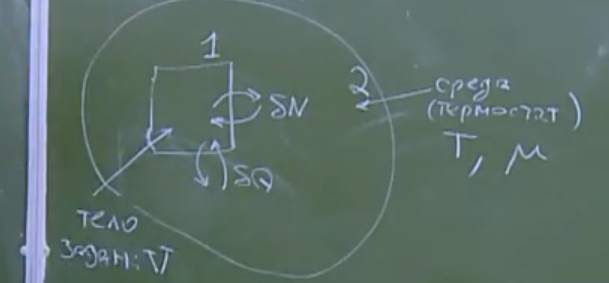
\includegraphics[width=0.4\textwidth]{images/2.png}
\end{center}

Тело 1 погружено в среду. Обозначим её индексом 2. Эту среду также называют термостатом или резервуаром. Среда очень большая, и она задает для нашего тела температуру $T$. Но теперь, поскольку возможен обмен частицами, среда задает еще одну важнейшую термодинамическую переменную — химический потенциал $\mu$. 

Между телом 1 и средой 2 происходит непрерывный обмен частицами и энергией (в форме теплоты). Теперь число частиц в теле $N_1$ не фиксировано. Это число непрерывно флуктуирует около какого-то среднего значения $\langle N_1 \rangle$. И именно это среднее значение будет определяться химическим потенциалом термостата.

При этом составная система «тело + среда» (система 1+2) является замкнутой. Она изолирована от остального мира и находится в состоянии термодинамического равновесия. Раз она замкнутая, мы можем сказать, что статистический оператор для всей этой огромной системы есть просто матрица плотности микроканонического распределения. 

Обозначим число частиц в теле как $N_1$, а в среде как $N_2$. Поскольку полная система замкнута, суммарное число частиц строго фиксировано:
\begin{equation*}
    N_1 + N_2 = N = \text{const}
\end{equation*}
Аналогично, полная энергия системы строго зафиксирована (с точностью до узкого слоя $\Delta E$):
\begin{equation*}
    E_1 + E_2 = E = \text{const}
\end{equation*}
Гамильтониан всей системы $\hat{H}$ складывается из гамильтонианов подсистем:
\begin{equation*}
    \hat{H} = \hat{H}_1 + \hat{H}_2
\end{equation*}
Мы предполагаем, что взаимодействие между телом и средой слабое. Оно не входит явно в гамильтониан, но оно обязательно присутствует, чтобы обеспечивать установление равновесия.

Пусть тело находится в некотором квантовом состоянии $|\Psi_{k_1, N_1}\rangle$ с энергией $E_{k_1, N_1}$. Индекс $k_1$ нумерует квантовые состояния тела при заданном числе частиц $N_1$. Среда находится в квантовом состоянии $|\Psi_{k_2, N_2}\rangle$ с энергией $E_{k_2, N_2}$. 

% --- SUBSECTION: Разложение энтропии среды по малому изменению энергии и числа частиц ---
\subsection{Разложение энтропии среды по малому изменению энергии и числа частиц}

Наша задача — найти вероятность $w_{k_1, N_1}$ того, что мы обнаружим наше тело именно в квантовом состоянии $k_1$ с числом частиц $N_1$. 

Для микроканонического ансамбля полной системы эта вероятность пропорциональна числу доступных микросостояний среды, при которых полная энергия сохраняется. То есть мы должны просуммировать по всем состояниям среды $k_2$, удовлетворяющим закону сохранения энергии:
\begin{equation*}
    E_{k_1, N_1} + E_{k_2, N_2} \leq E + \Delta E
\end{equation*}
Сумма $\sum_{k_2} 1$ по всем таким доступным состояниям термостата — это, по определению, статистический вес среды $\Omega_2$, вычисленный при энергии $E - E_{k_1, N_1}$ и числе частиц $N - N_1$. 

Таким образом, искомая вероятность пропорциональна статвесу среды:
\begin{equation*}
    w_{k_1, N_1} = \frac{\Omega_2(E - E_{k_1, N_1}, N - N_1)}{\Omega(E, N)}
\end{equation*}
где $\Omega(E, N)$ — полный статистический вес системы (константа нормировки).

Поскольку статвес среды — это экспонента от ее энтропии ($\Omega_2 = e^{S_2}$), перейдем к энтропии:
\begin{equation*}
    S_2(E - E_1, N - N_1) = \ln \Omega_2(E - E_1, N - N_1)
\end{equation*}
(Здесь и далее для краткости обозначим $E_{k_1, N_1}$ просто как $E_1$). 

Мы используем тот факт, что наше тело макроскопически мало по сравнению с термостатом. Это означает, что $E_1 \ll E$ и $N_1 \ll N$. Разложим энтропию среды $S_2$ в ряд Тейлора по малым параметрам $E_1$ и $N_1$, ограничившись линейными членами:
\begin{equation}
    S_2(E - E_1, N - N_1) \approx S_2(E, N) - \frac{\partial S_2}{\partial E} E_1 - \frac{\partial S_2}{\partial N} N_1
\end{equation}

Вспомним термодинамические определения производных энтропии. Производная энтропии по энергии — это обратная температура:
\begin{equation*}
    \frac{\partial S_2}{\partial E} = \frac{1}{T_2} = \frac{1}{T}
\end{equation*}
(Температура среды $T_2$ равна температуре тела $T$ в состоянии теплового равновесия).

Производная энтропии по числу частиц выражается через химический потенциал:
\begin{equation*}
    \frac{\partial S_2}{\partial N} = -\frac{\mu_2}{T_2} = -\frac{\mu}{T}
\end{equation*}

Подставляя эти производные в разложение, получаем:
\begin{equation}
    S_2(E - E_1, N - N_1) \approx S_2(E, N) - \frac{E_1}{T} + \frac{\mu N_1}{T}
\end{equation}

% --- SUBSECTION: Вероятность обнаружить систему в заданном микросостоянии ---
\subsection{Вероятность обнаружить систему в заданном микросостоянии}

Возвращаясь от энтропии обратно к статистическому весу (потенцируя), находим:
\begin{equation*}
    \Omega_2(E - E_1, N - N_1) \approx \Omega_2(E, N) \exp\left( \frac{\mu N_1 - E_1}{T} \right)
\end{equation*}

Подставляя это в выражение для вероятности, мы видим, что множитель $\frac{\Omega_2(E, N)}{\Omega(E, N)}$ зависит только от полных параметров системы $E$ и $N$ и не зависит от микросостояния тела. Его можно обозначить как новую нормировочную константу $1/\mathcal{Z}$. 

Опуская индекс «1», так как мы теперь говорим только о нашем исследуемом теле, мы получаем финальную формулу для вероятности обнаружить систему в квантовом состоянии $k$ с числом частиц $N$:
\begin{equation}
    w_{k, N} = \frac{1}{\mathcal{Z}} \exp\left( \frac{\mu N - E_{k, N}}{T} \right)
    \label{eq:grand_canonical_prob}
\end{equation}
Это и есть Большое каноническое распределение Гиббса.

% --- SUBSECTION: Введение большой статистической суммы ---
\subsection{Введение большой статистической суммы}

Константа нормировки $\mathcal{Z}$ находится из условия, что сумма всех вероятностей по всем возможным числам частиц $N$ и всем возможным квантовым состояниям $k$ (при данном $N$) должна равняться единице:
\begin{equation*}
    \sum_N \sum_k w_{k, N} = 1
\end{equation*}
Отсюда мы получаем определение величины $\mathcal{Z}$, которая называется \textbf{большой статистической суммой}:
\begin{equation}
    \mathcal{Z} = \sum_{N=0}^{\infty} \sum_k \exp\left( \frac{\mu N - E_{k, N}}{T} \right)
    \label{eq:grand_partition_function}
\end{equation}
Обратите внимание на структуру: мы сначала суммируем по всем квантовым состояниям $k$ при заданном числе частиц $N$, а затем суммируем по всем возможным значениям числа частиц от нуля до бесконечности.

% --- SUBSECTION: Статистический оператор Большого канонического ансамбля ---
\subsection{Статистический оператор Большого канонического ансамбля}

Как выглядит статистический оператор для большого канонического распределения? Сразу отсюда мы вспоминаем статистический оператор. Чему он равен? Статистический оператор $\hat{\rho}$ есть сумма для большого канонического распределения по всем $k$ и $N$:
\begin{equation*}
    \hat{\rho} = \sum_{k, N} w_{k, N} |\Psi_{k, N}\rangle \langle \Psi_{k, N}|
\end{equation*}
Во что свертывается этот оператор? Если я сюда подставлю найденную вероятность $w_{k, N} = \frac{1}{\mathcal{Z}} e^{\frac{\mu N - E_{k, N}}{T}}$, то выражение примет вид:
\begin{equation*}
    \hat{\rho} = \sum_{k, N} \frac{1}{\mathcal{Z}} e^{\frac{\mu N - E_{k, N}}{T}} |\Psi_{k, N}\rangle \langle \Psi_{k, N}|
\end{equation*}

Посмотрим на действие операторов. Если я подействую выражением $\frac{1}{\mathcal{Z}} e^{\frac{\mu \hat{N} - \hat{H}}{T}}$ на волновую функцию $|\Psi_{k, N}\rangle$, что это такое есть? Это есть ни что иное, как оператор, действующий на свою собственную функцию. Поскольку волновые функции $|\Psi_{k, N}\rangle$ — это собственные функции оператора числа частиц $\hat{N}$ (с собственным значением $N$) и гамильтониана $\hat{H}$ (с собственным значением $E_{k, N}$), вы получите ровно этот же числовой экспоненциальный фактор. 

Тогда вы можете заменить числа в экспоненте на операторы и вынести этот общий операторный множитель за знак суммы:
\begin{equation*}
    \hat{\rho} = \frac{1}{\mathcal{Z}} e^{\frac{\mu \hat{N} - \hat{H}}{T}} \sum_{k, N} |\Psi_{k, N}\rangle \langle \Psi_{k, N}|
\end{equation*}
А здесь у вас образуется сумма по $k$ и $N$ вот таких символов (проекторов) $|\Psi_{k, N}\rangle \langle \Psi_{k, N}|$. Что это такое есть? Единица. Это полный набор состояний. Сумма проекторов на все возможные состояния дает единичный оператор $\hat{1}$. 

Поэтому в результате вы получаете, что статистический оператор $\hat{\rho}$ для большого канонического распределения имеет исключительно компактный вид:
\begin{equation}
    \hat{\rho} = \frac{1}{\mathcal{Z}} e^{\frac{\mu \hat{N} - \hat{H}}{T}}
\end{equation}

Ну а большая статсумма $\mathcal{Z}$, соответственно, находится из условия нормировки $\operatorname{Sp}(\hat{\rho}) = 1$ и равна шпуру от этой экспоненты:
\begin{equation}
    \mathcal{Z} = \operatorname{Sp} \left( e^{\frac{\mu \hat{N} - \hat{H}}{T}} \right)
\end{equation}
Итак, вот мы получили выражение для статистического оператора и для статсуммы в терминах квантовой статистики.

Ну и еще один момент, который я хотел бы здесь сказать. Что подразумевается под суммой $\sum_{k, N}$? Что подразумевается под суммой по $k$ и $N$?
\begin{equation*}
    \sum_{k, N} \equiv \sum_{N=0}^{\infty} \sum_k
\end{equation*}
Что подразумевается? Сумма по всем квантовым состояниям и всем числам частиц. Это означает, что вы суммируете по всем $N$ формально от нуля до бесконечности, и при заданном числе частиц вы суммируете по всем квантовым состояниям $k$. По всем квантовым состояниям, возможным при заданном числе частиц. Вот вы задали $N$ — и пошли бесконечную сумму считать. Задали другое $N$ — и пошли бесконечную сумму считать. Вот, вообще говоря, нетривиальные такие суммы.




% --- SECTION: Термодинамические следствия Большого канонического ансамбля ---
\section{Термодинамические следствия Большого канонического ансамбля}

Как с этим распределением работать? Давайте начнем потихоньку привыкать. 

% --- SUBSECTION: Вычисление среднего числа частиц системы ---
\subsection{Вычисление среднего числа частиц системы}

Если нам надо посчитать среднее для какой-то физической величины $A$ в квантовой механике, ей соответствует некий эрмитов оператор $\hat{A}$. В каждой физической величине задается соответствующий оператор, и чтобы найти её среднее значение, мы должны взять шпур от произведения оператора этой величины на матрицу плотности: $\langle A \rangle = \operatorname{Sp}(\hat{A}\hat{\rho})$.

Давайте вычислим простейшую величину — среднее число частиц в нашей системе. Что я должен сделать? Я должен просуммировать по всем $k$ и $N$. В качестве оператора мы берем оператор числа частиц $\hat{N}$ и вычисляем его квантовомеханическое среднее в заданном состоянии, а затем умножаем на вероятность этого состояния:
\begin{equation*}
    \langle N \rangle = \sum_{k, N} \langle \Psi_{k, N} | \hat{N} | \Psi_{k, N} \rangle w_{k, N}
\end{equation*}

Оператор числа частиц $\hat{N}$, действуя на свою собственную волновую функцию $|\Psi_{k, N}\rangle$, просто дает собственное значение $N$. Волновая функция нормирована на единицу ($\langle \Psi_{k, N} | \Psi_{k, N} \rangle = 1$), поэтому квантовомеханическое среднее равно $N$. В результате мы получаем:
\begin{equation*}
    \langle N \rangle = \sum_{k, N} N w_{k, N}
\end{equation*}

Теперь подставим сюда явное выражение для вероятности $w_{k, N}$ в большом каноническом ансамбле, которое мы только что получили:
\begin{equation*}
    \langle N \rangle = \sum_{k, N} N \frac{1}{\mathcal{Z}} \exp\left( \frac{\mu N - E_{k, N}}{T} \right)
\end{equation*}

Посмотрим внимательно на это выражение. Я вижу, что комбинацию $N \exp\left( \frac{\mu N - E_{k, N}}{T} \right)$ я могу представить как производную от самой экспоненты по химическому потенциалу $\mu$, умноженную на температуру $T$. Действительно, при дифференцировании экспоненты по $\mu$ «спускается» множитель $N/T$. Чтобы скомпенсировать деление на температуру, нужно умножить производную на $T$. Поэтому я могу переписать выражение так, вынеся оператор дифференцирования за знак суммы:
\begin{equation*}
    \langle N \rangle = \frac{1}{\mathcal{Z}} T \frac{\partial}{\partial \mu} \sum_{k, N} \exp\left( \frac{\mu N - E_{k, N}}{T} \right)
\end{equation*}

Но сумма, стоящая под знаком производной, есть не что иное, как сама большая статистическая сумма $\mathcal{Z}$. Следовательно, мы получаем очень изящный результат:
\begin{equation}
    \langle N \rangle = \frac{T}{\mathcal{Z}} \frac{\partial \mathcal{Z}}{\partial \mu} = T \frac{\partial \ln \mathcal{Z}}{\partial \mu}
    \label{eq:mean_N_derivative}
\end{equation}
Это исключительно полезная формула. Зная большую статсумму как функцию температуры, объема и химического потенциала, мы простым дифференцированием по химическому потенциалу сразу находим среднее число частиц в системе.

% --- SUBSECTION: Связь большой статсуммы с термодинамикой: Большой потенциал ---
\subsection{Связь большой статсуммы с термодинамикой: Большой потенциал}

Теперь следующий важный пункт: связь большой статсуммы $\mathcal{Z}$ с термодинамикой. 

Давайте рассмотрим энтропию Гиббса для большого канонического распределения. По определению, энтропия Гиббса — это среднее значение логарифма функции распределения, взятое с обратным знаком:
\begin{equation*}
    S = -\langle \ln w \rangle
\end{equation*}

Вычислим логарифм нашей вероятности $w_{k, N}$:
\begin{equation*}
    \ln w_{k, N} = -\ln \mathcal{Z} + \frac{\mu N}{T} - \frac{E_{k, N}}{T}
\end{equation*}

Теперь нам нужно усреднить это выражение по всем состояниям. Подставляем логарифм в определение энтропии:
\begin{equation*}
    S = - \sum_{k, N} w_{k, N} \left( -\ln \mathcal{Z} + \frac{\mu N}{T} - \frac{E_{k, N}}{T} \right)
\end{equation*}

Разобьем эту сумму на три слагаемых. 
Первое слагаемое: логарифм статсуммы $\ln \mathcal{Z}$ является константой (он не зависит от индексов суммирования $k$ и $N$), поэтому мы выносим его за знак суммы. Оставшаяся сумма вероятностей $\sum w_{k, N}$ равна единице по условию нормировки. Значит, первое слагаемое дает просто $\ln \mathcal{Z}$.

Второе слагаемое содержит множитель $\mu / T$, который также выносится за сумму. Под суммой остается $\sum N w_{k, N}$, что, как мы только что выяснили, есть среднее число частиц $\langle N \rangle$.

Третье слагаемое содержит множитель $-1/T$. Оставшаяся под суммой величина $\sum E_{k, N} w_{k, N}$ по определению представляет собой среднюю энергию системы $\langle E \rangle$.

Собирая все вместе (и учитывая общий знак минус перед скобками), мы получаем:
\begin{equation*}
    S = \ln \mathcal{Z} - \frac{\mu \langle N \rangle}{T} + \frac{\langle E \rangle}{T}
\end{equation*}

Домножим обе части этого уравнения на температуру $T$:
\begin{equation*}
    TS = T \ln \mathcal{Z} - \mu \langle N \rangle + \langle E \rangle
\end{equation*}

Перегруппируем слагаемые, оставив член с логарифмом статсуммы слева:
\begin{equation*}
    -T \ln \mathcal{Z} = \langle E \rangle - TS - \mu \langle N \rangle
\end{equation*}

Давайте внимательно посмотрим на правую часть. Выражение $\langle E \rangle - TS$ в термодинамике представляет собой свободную энергию Гельмгольца $F$. В термодинамическом пределе мы можем опустить скобки усреднения, так как флуктуации малы, и писать просто $E$ и $N$. Таким образом, мы имеем:
\begin{equation*}
    -T \ln \mathcal{Z} = F - \mu N
\end{equation*}

Комбинация $F - \mu N$ представляет собой новый термодинамический потенциал. В статистической физике и термодинамике он называется \textbf{Большим термодинамическим потенциалом} или \textbf{Омега-потенциалом}. Мы будем обозначать его большой греческой буквой $\Omega$. Следовательно, мы приходим к фундаментальной связи:
\begin{equation}
    \Omega(T, V, \mu) = -T \ln \mathcal{Z}
    \label{eq:omega_potential_def}
\end{equation}
Это соотношение позволяет нам, вычислив большую статистическую сумму, мгновенно получить Омега-потенциал, который содержит в себе всю термодинамическую информацию об открытой системе.

% --- SUBSECTION: Дифференциал большого термодинамического потенциала ---
\subsection{Дифференциал большого термодинамического потенциала}

Давайте убедимся, что Омега-потенциал действительно удобен для работы. Запишем его дифференциал. По определению:
\begin{equation*}
    \Omega = F - \mu N
\end{equation*}
Берем полный дифференциал от обеих частей:
\begin{equation*}
    d\Omega = dF - d(\mu N)
\end{equation*}
Подставляем известное из термодинамики выражение для дифференциала свободной энергии $dF = -S dT - P dV + \mu dN$ и раскрываем дифференциал произведения:
\begin{equation*}
    d\Omega = (-S dT - P dV + \mu dN) - \mu dN - N d\mu
\end{equation*}
Слагаемые $\mu dN$ и $-\mu dN$ благополучно сокращаются, и у нас остается:
\begin{equation}
    d\Omega = -S dT - P dV - N d\mu
    \label{eq:dOmega}
\end{equation}

Из этого дифференциала мы сразу видим, что естественными независимыми переменными для потенциала $\Omega$ являются именно температура $T$, объем $V$ и химический потенциал $\mu$. Это в точности те параметры, которыми задается наш большой канонический ансамбль! 

Также из выражения для дифференциала немедленно следуют формулы для вычисления сопряженных величин через частные производные:
\begin{align*}
    S &= -\left( \frac{\partial \Omega}{\partial T} \right)_{V, \mu} \\
    P &= -\left( \frac{\partial \Omega}{\partial V} \right)_{T, \mu} \\
    N &= -\left( \frac{\partial \Omega}{\partial \mu} \right)_{T, V}
\end{align*}

Посмотрите на последнюю формулу: $N = -\left( \frac{\partial \Omega}{\partial \mu} \right)_{T, V}$. Если мы подставим сюда $\Omega = -T \ln \mathcal{Z}$, мы получим:
\begin{equation*}
    N = -\frac{\partial}{\partial \mu} (-T \ln \mathcal{Z}) = T \frac{\partial \ln \mathcal{Z}}{\partial \mu}
\end{equation*}
Это в точности совпадает с выражением \eqref{eq:mean_N_derivative}, которое мы строго вывели из микроскопического усреднения! Термодинамика и статистическая механика находятся в полном согласии.

% --- SUBSECTION: Вывод уравнения состояния (Омега-потенциал и давление) ---
\subsection{Вывод уравнения состояния (Омега-потенциал и давление)}

Второе свойство этого потенциала немного похитрее, но оно очень красивое. Давайте зададимся вопросом: какая величина сам Омега-потенциал $\Omega(T, V, \mu)$? Очевидно, что это величина экстенсивная, то есть она должна быть прямо пропорциональна размерам системы. 

Из переменных $T, V, \mu$ экстенсивной величиной является только объем $V$. Температура и химический потенциал — величины интенсивные. Следовательно, из соображений размерности и аддитивности, Омега-потенциал обязан быть прямо пропорционален объему:
\begin{equation*}
    \Omega \sim V
\end{equation*}
Это означает, что мы можем представить $\Omega$ в виде произведения объема на некую функцию, зависящую только от интенсивных параметров:
\begin{equation*}
    \Omega = V \cdot \omega(T, \mu)
\end{equation*}
где $\omega(T, \mu)$ — это плотность Омега-потенциала (Омега-потенциал на единицу объема).

А теперь давайте возьмем частную производную от $\Omega$ по объему при постоянных $T$ и $\mu$. Из структуры $\Omega = V \cdot \omega(T, \mu)$ очевидно, что:
\begin{equation*}
    \left( \frac{\partial \Omega}{\partial V} \right)_{T, \mu} = \omega(T, \mu) = \frac{\Omega}{V}
\end{equation*}
С другой стороны, из дифференциала \eqref{eq:dOmega} мы знаем термодинамическое определение этой производной:
\begin{equation*}
    \left( \frac{\partial \Omega}{\partial V} \right)_{T, \mu} = -P
\end{equation*}
Приравнивая эти два выражения, мы получаем:
\begin{equation*}
    \frac{\Omega}{V} = -P
\end{equation*}
Или, переписывая окончательно:
\begin{equation}
    \Omega = -PV
    \label{eq:Omega_PV}
\end{equation}
Это означает, что Омега-потенциал с точностью до знака равен произведению давления на объем. Это исключительно мощное утверждение. Вычисляя большую статсумму, вы находите $\Omega$, а значит, сразу же находите уравнение состояния системы, так как давление $P = -\Omega/V = (T/V) \ln \mathcal{Z}$.

% --- SUBSECTION: Связь химического потенциала и удельного термодинамического потенциала ---
\subsection{Связь химического потенциала и удельного термодинамического потенциала}

И еще один пример, где появляется подобная величина, который полезно рассмотреть в контексте свойств экстенсивности. Давайте вспомним термодинамический потенциал Гиббса (энергию Гиббса), который обозначается буквой $\Phi$. По определению:
\begin{equation*}
    \Phi = E - TS + PV = F + PV
\end{equation*}
Его дифференциал имеет вид:
\begin{equation*}
    d\Phi = -S dT + V dP + \mu dN
\end{equation*}
Отсюда видно, что естественными переменными для энергии Гиббса являются $(T, P, N)$. Функция $\Phi(T, P, N)$ тоже является экстенсивной величиной, поэтому она должна быть пропорциональна единственной экстенсивной переменной в этом наборе, то есть числу частиц $N$:
\begin{equation*}
    \Phi = N \cdot \varphi(T, P)
\end{equation*}
где $\varphi(T, P)$ — удельный термодинамический потенциал на одну частицу.

С другой стороны, из дифференциала энергии Гиббса следует, что частная производная $\Phi$ по числу частиц дает химический потенциал:
\begin{equation*}
    \left( \frac{\partial \Phi}{\partial N} \right)_{T, P} = \mu
\end{equation*}
Беря производную от выражения $\Phi = N \cdot \varphi(T, P)$ по $N$, мы получаем просто $\varphi(T, P)$. Следовательно:
\begin{equation*}
    \varphi(T, P) = \mu(T, P)
\end{equation*}
Подставляя это обратно, мы находим, что полная энергия Гиббса есть просто произведение числа частиц на химический потенциал:
\begin{equation}
    \Phi = \mu N
    \label{eq:Phi_muN}
\end{equation}
Это соотношение тоже очень полезно помнить. Оно показывает, что химический потенциал — это не что иное, как удельная энергия Гиббса, приходящаяся на одну частицу.

Вот такая хитрость этого распределения. Использование открытой системы и переход к флуктуирующему числу частиц делает математический аппарат невероятно гибким. Если бы вы пытались наложить жесткие ограничения, вы бы замучались считать эти суммы, а ослабив связи, мы получаем элегантные и точные результаты.

На этом мы ставим точку. В следующий раз мы применим этот мощный аппарат для описания квантовых идеальных систем — газов Бозе и Ферми, и увидим всю красоту квантовой статистики в действии. На сегодня всё, всем спасибо.


\end{document}
